\documentclass[10pt]{beamer}
% Beamer uses a standard paper size of 128x96mm

% ===== Packages =====
\usepackage[utf8]{inputenc}
\usepackage[T1]{fontenc}

\usepackage{graphicx}
\usepackage{tikz}  % TODO: utilisé pourquoi? (il est particulierement lent a compiler avec)
\usepackage{enumitem} % Custom lists
\usepackage{mathtools} % endlesssssss maths

\usepackage[backend=biber, autolang=other, style=phys, sorting=none]{biblatex}  % Citing
\addbibresource{../bibliography/bibliography.bib}
\makeatletter
\renewcommand\@makefnmark{\hbox{{\usebeamercolor[fg]{footnote mark}\usebeamerfont*{footnote mark}[\@thefnmark]}}}     %% to replace "[#1]" with "(#1)"
\makeatother
% ===== Typeface =====
\usepackage{mlmodern} % thicker math, do not touch

% \usepackage[sfdefault]{FiraSans} % peculiar but nice
% \usepackage{tgheros} % nice
\usepackage[sfdefault]{plex-sans} % nice
% \usepackage[sfdefault]{noto}
% \usepackage[sfdefault, light]{FiraSans} 
% \usepackage{helvet}
% \usepackage[sfdefault]{AlegreyaSans} % peculiar
% \usepackage{montserrat}
% \usepackage{raleway}
% \usepackage{avant} % nah
% \usepackage{tgadventor} % nah
% \usepackage{cmbright} % meh
% \usepackage{DejaVuSans} % big
% https://tug.org/FontCatalogue/sansseriffonts.html

% ===== Beamer theme =====
\usetheme{Boadilla} % other interesting built-in: Boadilla, CambridgeUS (if we want sections in header), Pittsburgh (super-plain)

\setbeamertemplate{footline}{   % only page number in footline
\hfill%
\usebeamercolor[fg]{page number in head/foot}%
% \usebeamerfont{page number in head/foot}%
\footnotesize%
    \setbeamertemplate{page number in head/foot}[framenumber]%
    \usebeamertemplate*{page number in head/foot}\kern0.5em\vskip4pt%
    }
    \addtobeamertemplate{footline}{\vspace*{-0.5cm}}{}
    
    \setbeamertemplate{blocks}[rounded][shadow=false]
    \setbeamertemplate{navigation symbols}{}

    
% ===== Colors =====
% \usecolortheme{beaver}
\definecolor{UBCblue}{rgb}{0.04706, 0.13725, 0.26667} % UBC Blue (primary)
% \definecolor{EPFLred}{RGB}{255, 0, 0}
\definecolor{darkred}{rgb}{0.7,0,0}

\usecolortheme[named=UBCblue]{structure}

% \setbeamercolor{block title}{bg=cyan!50, fg=white} % modifying colors (the ! is for trasparency)

% \setbeamercolor{section in toc}{fg=black,bg=white}
% \setbeamercolor{alerted text}{fg=darkred!80!gray}
% \setbeamercolor*{palette primary}{fg=darkred!60!black,bg=gray!30!white}
% \setbeamercolor*{palette secondary}{fg=darkred!70!black,bg=gray!15!white}
% \setbeamercolor*{palette tertiary}{bg=darkred!80!black,fg=gray!10!white}
% \setbeamercolor*{palette quaternary}{fg=darkred,bg=gray!5!white}

% \setbeamercolor*{sidebar}{fg=darkred,bg=gray!15!white}

% \setbeamercolor*{palette sidebar primary}{fg=darkred!10!black}
% \setbeamercolor*{palette sidebar secondary}{fg=white}
% \setbeamercolor*{palette sidebar tertiary}{fg=darkred!50!black}
% \setbeamercolor*{palette sidebar quaternary}{fg=gray!10!white}

% \setbeamercolor*{titlelike}{parent=palette primary}
\setbeamercolor{titlelike}{fg=black}
\setbeamercolor{frametitle}{fg=black}
% \setbeamercolor{frametitle right}{bg=gray!60!white}

% \setbeamercolor*{separation line}{}
% \setbeamercolor*{fine separation line}{}

% \definecolor{cyanish}{RGB}{10,250,250}  % different ways to define colors
% \definecolor{lightgreen}{HTML}{CCFF99}
% \definecolor{orangish}{wave}{620}
% \colorlet{ochre}{blue!30!yellow!70!}

% ===== Text properties =====
\renewcommand*\familydefault{\sfdefault} % sans-serif as default
% \linespread{1.3} % Change line spacing
\usefonttheme{professionalfonts} % uses Computer Modern for math as God intended
\setbeamerfont{bibliography entry author}{size=\scriptsize, series=\normalfont} 
\setbeamerfont{bibliography entry title}{size=\scriptsize, series=\bfseries} 
\setbeamerfont{bibliography entry location}{size=\scriptsize, series=\normalfont} 

% ===== Avoid footnotes at the end of columns =====
\makeatletter
\renewrobustcmd{\blx@mkbibfootnote}[2]{%
\iftoggle{blx@footnote}
{\blx@warning{Nested notes}%
\addspace\mkbibparens{#2}}
{\unspace
\ifnum\blx@notetype=\tw@
\expandafter\@firstoftwo
\else
\expandafter\@secondoftwo
\fi
{\csuse{blx@theendnote#1}{\protecting{\blxmkbibnote{end}{#2}}}}
{\csuse{footnote#1}[frame]{\protecting{\blxmkbibnote{foot}{#2}}}}}}
\makeatother
% \setlist[itemize]{label={$\vcenter{\hbox{\scriptsize$\bullet$}}$}, leftmargin=0.6cm, topsep=-3pt}
\setlist[itemize]{label={--}, leftmargin=0.6cm}

% ===== Global background =====
% %Global Background must be put in preamble
% \usebackgroundtemplate%
% {%
%     \includegraphics[width=\paperwidth,height=\paperheight]{newton.jpg}%
% }

% ===== Title logo =====
\titlegraphic { 
\begin{tikzpicture}[overlay,remember picture]
\node[right=0.2cm] at (current page.147){
    
\includegraphics[width=1.5cm]{../figures/EPFL_logo.png}
};
\end{tikzpicture}
}
% Or more simply:
% \titlegraphic{
\includegraphics[width=1.5cm]{../figures/EPFL_logo.png}} % Title logo

% ===== Commands =====
\newcommand{\probecurrent}[0]{\ensuremath{I_{\mathrm{probe}}}}
\newcommand{\electronsaturationcurrent}[0]{\ensuremath{I_{e,{\mathrm{sat}}}}}
\newcommand{\biasvoltage}{\ensuremath{V_{\mathrm{bias}}}}
\newcommand{\probevoltage}{\ensuremath{V_{\mathrm{probe}}}}
\newcommand{\plasmavoltage}{\ensuremath{V_{\mathrm{plasma}}}}
\newcommand{\filamentcurrent}{\ensuremath{I_{\mathrm{filament}}}}
\newcommand{\filamentpolarisation}{\ensuremath{V_{\mathrm{filament}}}}
\newcommand{\gridpolarisation}{\ensuremath{V_{\mathrm{grid}}}}
\newcommand{\electron}[0]{$e^{-}$}

% ===== Presentation =====
\title{Argon plasma analysis using Langmuir probes}
\author{Tom Vadot \and Matteo Veneziano}
\institute{EPFL Section of Physics}
\date{November 29, 2024}
% \logo{
\includegraphics[width=1.5cm]{../figures/EPFL_logo.png}} % logo en chaque page

\begin{document}

\begin{frame}
    \titlepage
\end{frame}

\section{Introduction}
\begin{frame}{Introduction}
    Space stuff

    Langmuir on ISS

    Solar events

    Communication and GPS satelites

    \url{https://www.space.com/space-weather-sensors-heads-to-space-station}
    \url{https://www.esa.int/Science_Exploration/Human_and_Robotic_Exploration/Probe_the_space_weather_around_Earth}
    \url{https://www.esa.int/Enabling_Support/Space_Engineering_Technology/Shaping_the_Future/Multi-Needle_Langmuir_Probe_Tested_and_Ready_for_Launch}
    \url{https://www.esa.int/Science_Exploration/Human_and_Robotic_Exploration/Probe_the_space_weather_around_Earth}
    \url{https://www.esa.int/Education/ESEO/Langmuir_Probe}
\end{frame}

\section{Theory and experimental setup}
\begin{frame}{Defining plasma}
    A \emph{quasineutral} gas of charged and neutral particles which exhibit \emph{collective} behaviour" \footfullcite{chen_introduction_2006}
    \vspace{0.5cm}
    \begin{itemize}
        \item \textbf{Quasineutrality}: the overall charge densities of free electrons and ions cancel each other in equilibrium: 
            $n_e \simeq Z n_i$ \footfullcite{gibbon_introduction_2016}

        \item \textbf{Collective behaviour}: macroscopic fields dominate over short-lived microscopic fluctuations.
            An external stimulus creates a simultaneous response of many particles \footfullcite{piel_plasma_2017}.
    \end{itemize}
    \vspace{0.5cm}
    Cold plasma: ions are not thermalised and electrons have a temperature such that $T_e \gg T_i$ \footfullcite{bagnato_notice_2019}.
\end{frame}


\begin{frame}{Langmuir probes}
    \vspace{0.2cm}
    \begin{itemize}
        \item Devices widely used to study different properties of plasma, e.g. electron temperature $T_e$ and density $n_e$.
        
        \item Electrode of surface $A_{\mathrm{probe}}$, inserted into the chamber and biased by an external voltage $\biasvoltage$.
        \item The charges (both ions and electrons) reach the surface and generate probe current $\probecurrent = I_e + I_i$.
        \item Measuring the probe potential $\probevoltage$ yields the plasma space potential $\plasmavoltage$:
        \begin{equation*}
            \biasvoltage= \probevoltage - \plasmavoltage
        \end{equation*}
    \end{itemize}

    \begin{center}
        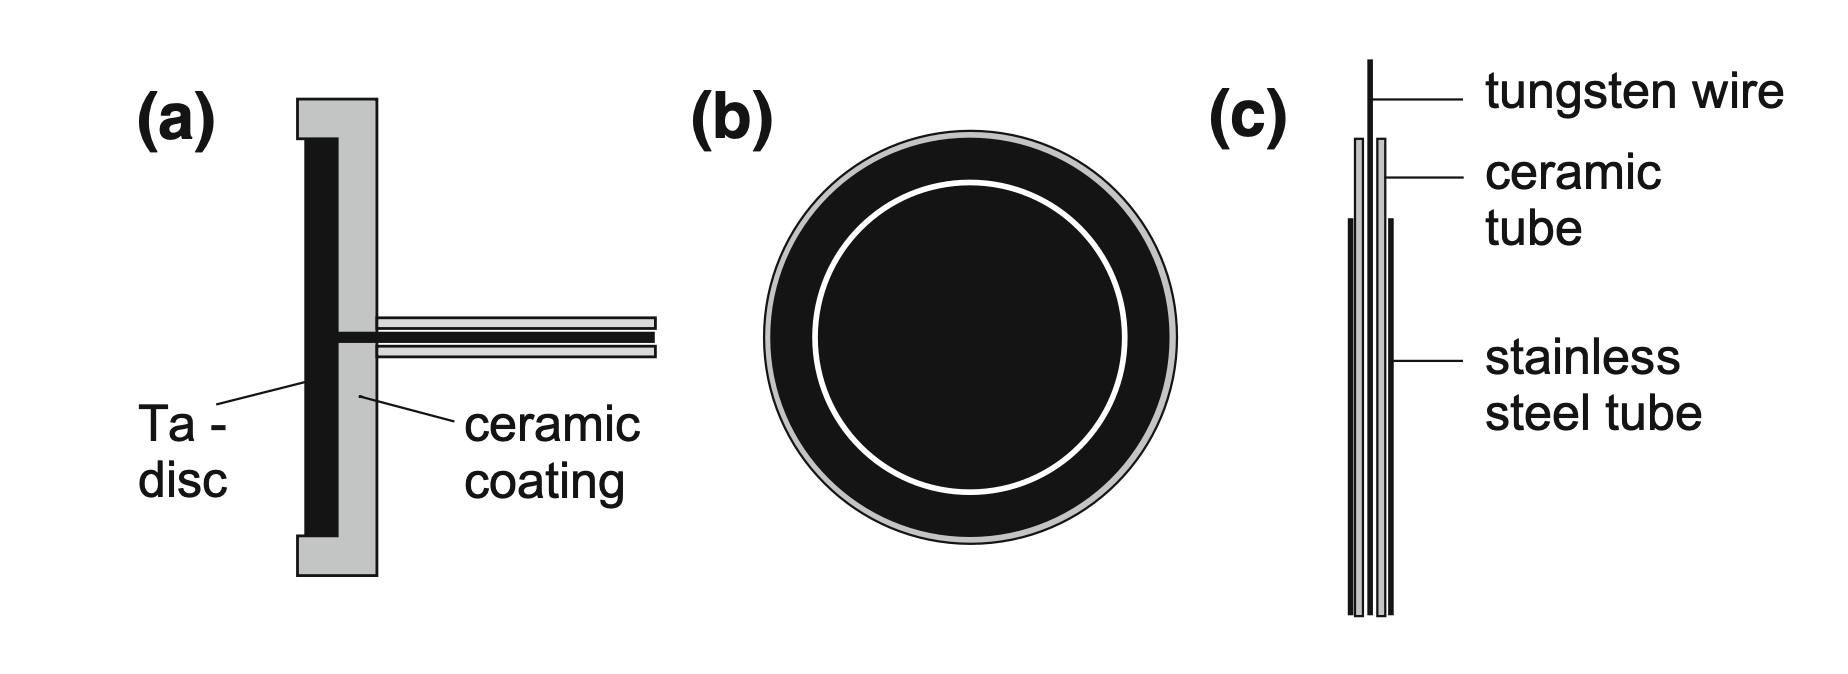
\includegraphics[width=0.65\textwidth]{../figures/langmuir_probe.png}
        \\
        \small Structure of a common plane Langmuir probe \footfullcite{piel_plasma_2017}
    \end{center}
\end{frame}


\begin{frame}{The $I$--$V$ characteristic curve}
    \begin{columns}
        \column{0.5\textwidth}
        Three regions:
        \begin{enumerate}
            \item[I] High negative bias: no electrons reach the probe. Constant ion saturation current.
            \item[II] Electron retardation regime: part of the electrons reach the probe. Electron current \footfullcite{bagnato_notice_2019}
            \begin{equation*}
                I_e = \electronsaturationcurrent \frac{e^{q(\probevoltage - \biasvoltage)}}{k_B T_e}
            \end{equation*}
            \item[III] High positive bias: constant electron saturation current $\electronsaturationcurrent$.
            \begin{equation*}
                \electronsaturationcurrent = \frac{1}{4}e n_e v_{e,th} A_{\mathrm{probe}}
            \end{equation*}
        \end{enumerate}
        \column{0.5\textwidth}
        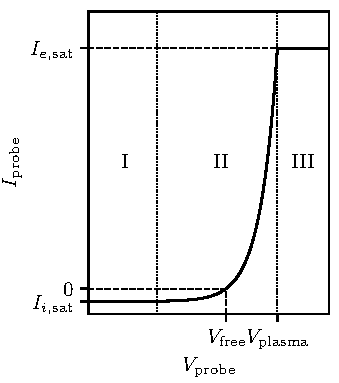
\includegraphics[scale=1]{../figures/langmuir_characteristic.pdf}
    \end{columns}
    % \begin{itemize}
    %     \item Floating potential $\Phi_f$: no current flows in the probe
    %     \item Plasma potential $\Phi_p$: the potential inside the ambient plasma, corresponds to $\electronsaturationcurrent$.
    % \end{itemize}
\end{frame}

\begin{frame}{Extracting electron temperature and density}
    \begin{columns}
        \column{0.5\textwidth}
        \begin{itemize}
            \item Acquire $I$-$V$ curve.
            \item Linearise region II.
            \item Linear regression in region II allows to find $T_e$.
                \begin{equation*}
                    \ln\left(\frac{I_e}{\electronsaturationcurrent} \right) = \frac{e}{k_B T_e}(\probevoltage - \biasvoltage)
                \end{equation*}
            \item Electron saturation current allows to find $n_e$
                \begin{equation*}
                    n_e = \frac{4}{e v_e A_p} \electronsaturationcurrent = \frac{1}{e A_p} \sqrt{\frac{2 \pi m_e}{k_B T_e}} \electronsaturationcurrent
                \end{equation*}
        \end{itemize}

         
        

        \column{0.5\textwidth}
        
\includegraphics[scale=1]{../figures/IV_fit.pdf}
    \end{columns}
\end{frame}

\begin{frame}{Experimental setup}
    % Prendre figure dans vieux rapport et citer?
    \centering
    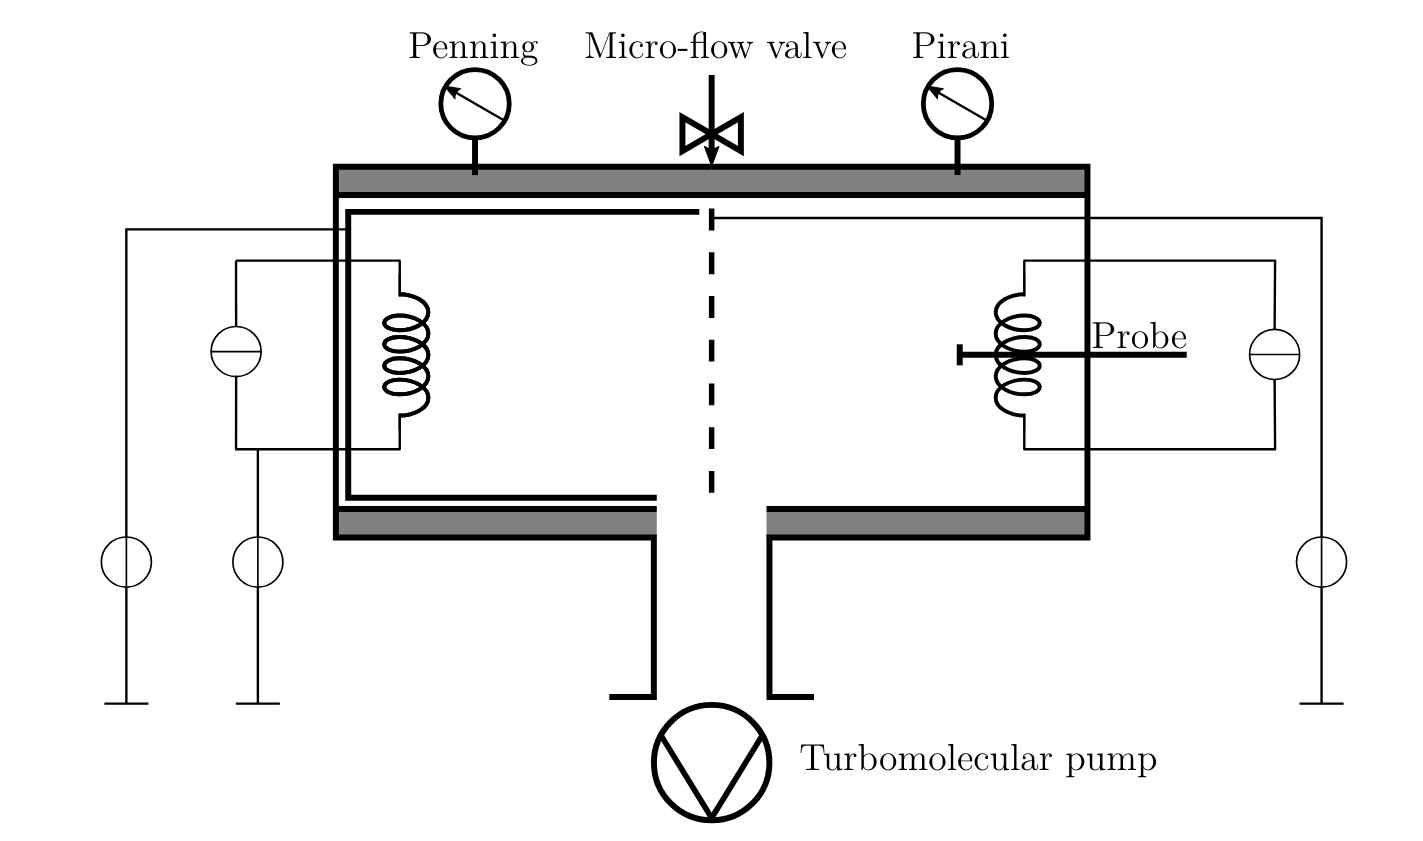
\includegraphics[width=\textwidth]{../figures/experimental_setup_Willemin_Zahar.png} 
    \\
    Diagram/schematics whatever of what we did\footfullcite{experimental_setup_Willemin_Zahar}
    % il est morlement impossible qua u fond ce brave monsieur ai tort
\end{frame}

\section{Results}
\begin{frame}{Temperature and density along the chamber axis}{$\filamentcurrent = (50.0 \pm 0.1)$ A, $\filamentpolarisation = (60 \pm 1)$ V, $\gridpolarisation = - (100 \pm 1)$ V}
    \begin{columns}[T]
        \column{0.5\textwidth}
        \centering
        {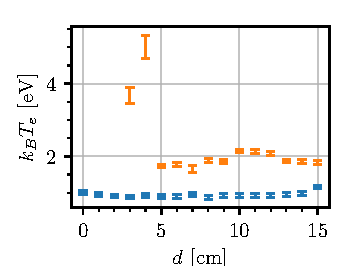
\includegraphics[scale=1]{../figures/temperatureeV_position.pdf}}
        \begin{itemize}
            \item Close to heating element and grid \(\rightarrow\) higher \electron temperature
            \item Higher pressure decreases temperature and increases density
            % \item Maximum of density 
            % \item Maximal density for distances $\sim 10$ cm from heating element
        \end{itemize}

        \column{0.5\textwidth}
        \centering
        {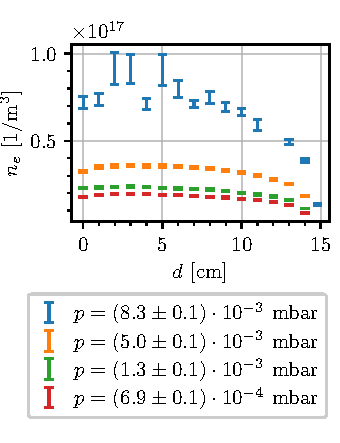
\includegraphics[scale=1]{../figures/density_position.pdf}}
    \end{columns}

\end{frame}
    
\begin{frame}{Effects of pressure}{$d = (3.0 \pm 0.5)$ cm, $\filamentcurrent = (49.9 \pm 0.1)$ A}

    \begin{columns}
        \column{0.5\textwidth}
        \centering
        {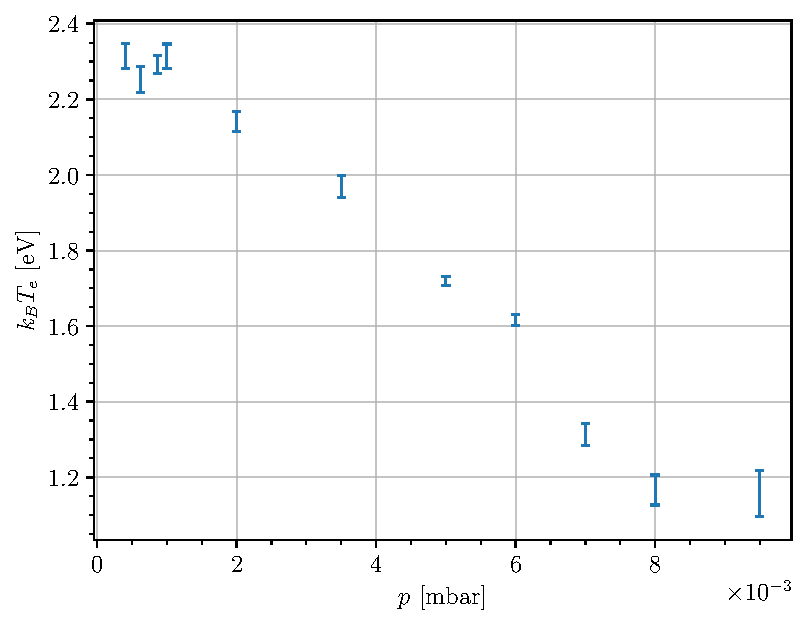
\includegraphics[scale=1]{../figures/temperatureeV_pressure.pdf}}


        \column{0.5\textwidth}
        \centering
        {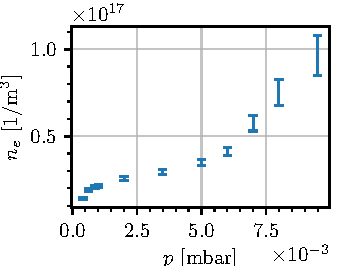
\includegraphics[scale=1]{../figures/density_pressure.pdf}}

    \end{columns}
    \begin{itemize}
        \item Higher pressure decreases temperature and decreases temperature.
        \item Non linear
    \end{itemize}
\end{frame}

\begin{frame}{Heating less}{$p = (4.2 \pm 0.1) \times 10^{-3}$ mbar, $d = (3.0 \pm 0.5)$ cm}
    \begin{columns}
        \column{0.5\textwidth}
        \centering
        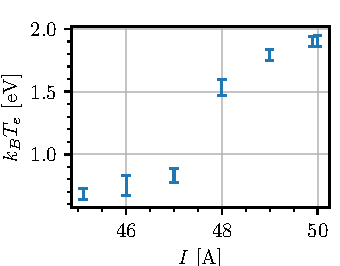
\includegraphics[scale=1]{../figures/temperatureeV_current.pdf}


        \column{0.5\textwidth}
        \centering
        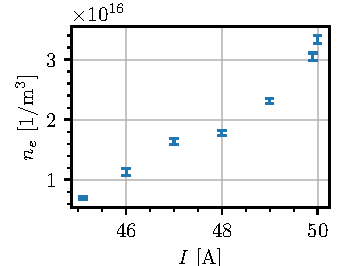
\includegraphics[scale=1]{../figures/density_current.pdf}

    \end{columns}
    \vspace{0.5cm}
    \begin{itemize}
        \item A higher filament current leads to more electrons emitted from the Tungsten and thus to higher temperature and density
        \item It was not possible to sustain a plasma at currents higher than $(50.0 \pm 0.1)$ A
    \end{itemize}
\end{frame}

% \begin{frame}{Variation avec filament polarisation}{IMPORTANT! donner les autres parametres (ceux qui n'ont pas été variés pour faire le plot)}
%     \begin{columns}
%         \column{0.5\textwidth}
%         \centering
%         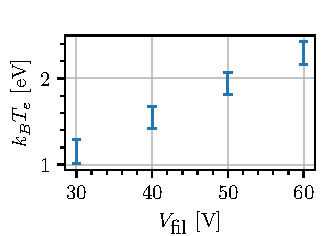
\includegraphics[scale=1]{../figures/temperatureeV_filament_polarisation.pdf}


%         \column{0.5\textwidth}
%         \centering
%         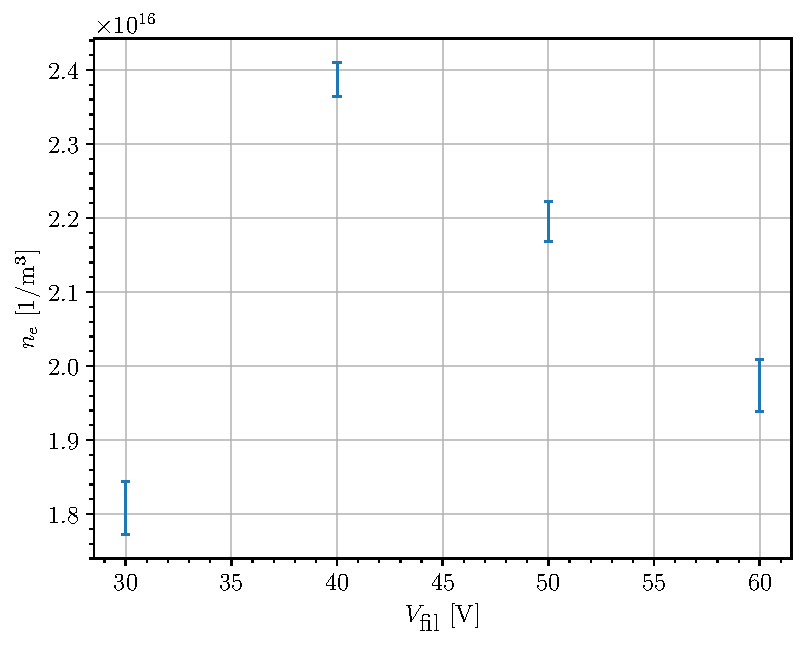
\includegraphics[scale=1]{../figures/density_filament_polarisation.pdf}

%     \end{columns}
%     \vspace{0.5cm}
%     \begin{itemize}
%         \item Temperature increases with polarisation
%         \item What is happening for density?
%     \end{itemize}
% \end{frame}

\begin{frame}{Radial Langmuir probe profile boh}
    \begin{columns}
        \column{0.5\textwidth}
        \centering
        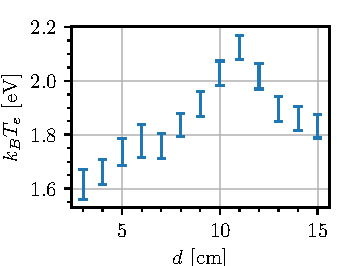
\includegraphics[scale=1]{../figures/temperatureeV_position_radial.pdf}

        \column{0.5\textwidth}
        \centering
        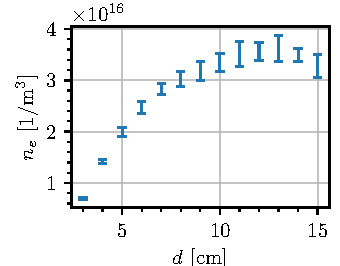
\includegraphics[scale=1]{../figures/density_position_radial.pdf}

    \end{columns}
    \vspace{0.5cm}
    Temperature and density falls off near the external walls.
\end{frame}



\begin{frame}{Temperature and density profile of the chamber}{$p = (9.5 \pm 0.1) \times 10^{-3}$ mbar, $\filamentcurrent = (50.0 \pm 0.1)$ A}
    \begin{columns}
        \column{0.5\textwidth}
        \centering
        {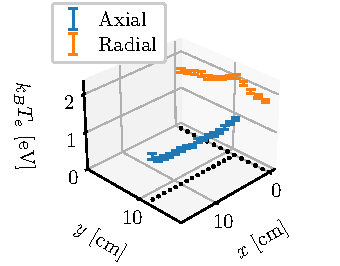
\includegraphics[scale=1]{../figures/temperatureEV_profile.pdf}}
        
        \column{0.5\textwidth}
        \centering
        {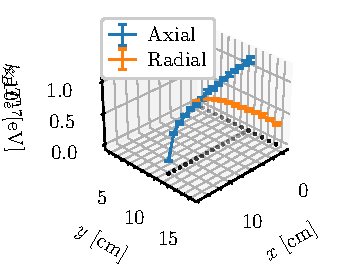
\includegraphics[scale=1]{../figures/density_profile.pdf}}
        
    \end{columns}
    \begin{itemize}
        \item The different orientation of the Langmuir probes leads to different results in the two halves of the chamber
        \item Density is highest closest to the filaments and to the cylinder axis
    \end{itemize}
\end{frame}

\begin{frame}{Turning off one filament}{$p = (1.3 \pm 0.1) \times 10^{-3}$ mbar, $\filamentcurrent = (50.0 \pm 0.1)$ A}
    \begin{columns}
        \column{0.5\textwidth}
        \centering
        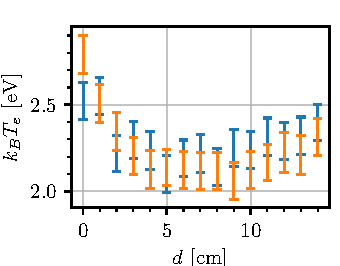
\includegraphics[scale=1]{../figures/temperatureeV_position_twofilaments.pdf}

        \column{0.5\textwidth}
        \centering
        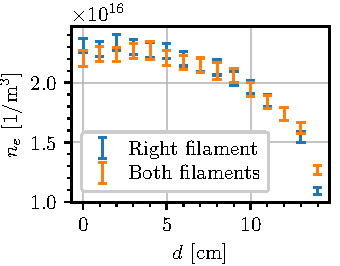
\includegraphics[scale=1]{../figures/density_position_twofilaments.pdf}

    \end{columns}
    \vspace{0.5cm}
    \begin{itemize}
        \item Only difference observed closest to the grid.
        \item No significant difference in the rest of the chamber, possibly due to the effect of the grid
    \end{itemize}
\end{frame}

\begin{frame}{Ion acoustic waves}
    \begin{itemize}
        \item Longitudal oscillation of charges in plasma
        \item Low pressure $\implies$ almost no collisions, only Coulomb interactions
        \item 1 type of ion: $_{18}$Ar
    \end{itemize}
    
    \vspace{0.5cm}
    \begin{columns}[T]
        \column{0.5\textwidth}
        Dispersion relation \space \footfullcite{bagnato_notice_2019}
        \begin{equation*}
            v_s^2 = \frac{\gamma_e Z_i k_B T_e + \gamma_i k_B T_i}{M(1+\gamma_e(k\lambda_d)^2)}
        \end{equation*}
        
        \column{0.01\textwidth}
        \rule{.1mm}{1.5cm}

        \column{0.49\textwidth}
        \vfill
        \centering
        $M$ mass of ion \\
        $Z$ charge of ion \\
        $T_e$/$T_i$ temperature of \electron/ion \\
        $\gamma_e=3$, $\gamma_i=1$
        \vfill
    \end{columns}

    \vspace{0.8cm}
    Under long wavelength and cold plasma assumption
    \begin{equation*}
        \begin{rcases}
            \lambda \gg \lambda_d \\
            T_i \ll 1
        \end{rcases}
        \implies v_s^2 = \frac{\gamma_e Z k_B T_e}{M}
    \end{equation*}

    Dispersionless assumption: $v_s = \frac{\omega}{k}$
\end{frame}

\begin{frame}{Estimating temperature}{$p = (7.1 \pm 0.1) \times 10^{-3}$ mbar, $I_\text{filament,left} = (49.7 \pm 0.1)$ A, $I_\text{filament,right} = (48.5 \pm 0.1)$ A, $V_\text{filament} = (-60 \pm 2)$ V, $V_\text{grid} = (-100 \pm 1)$ V}
    \begin{columns}
        \column{0.5\textwidth}
        \centering
        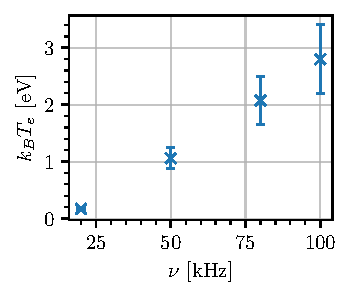
\includegraphics[scale=1]{../figures/ion_acoustic_temperature.pdf}
        \begin{itemize}
            \item Source wave not exactly replicated
            \item Unexpected temperature increase for higher source frequency
        \end{itemize}
        
        \column{0.5\textwidth}
        \centering
        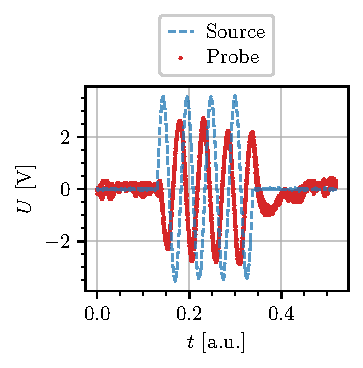
\includegraphics[scale=1]{../figures/ion_acoustic_wave.pdf}
    \end{columns}
\end{frame}

\begin{frame}{Establishing the dispersion relation}{$p = (7.1 \pm 0.1) \times 10^{-3}$ mbar, $I_\text{filament,left} = (49.7 \pm 0.1)$ A, $I_\text{filament,right} = (48.5 \pm 0.1)$ A, $V_\text{filament} = (-60 \pm 2)$ V, $V_\text{grid} = (-100 \pm 1)$ V}
    \begin{columns}
        \column{0.5\textwidth}
        \centering
        \vspace{-1cm}
        \begin{itemize}
            \item Very few data points due to unstable system
            \item Doesn't seem linear $\implies$ not dispersionless
            \item If dispersionless assumption does not hold, could explain the increasing temperature
        \end{itemize}
        
        \column{0.5\textwidth}
        \centering
        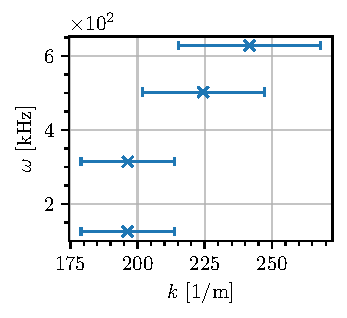
\includegraphics[scale=1]{../figures/dispersion_relation.pdf}
    \end{columns}
\end{frame}

\section{Discussion}
\begin{frame}{Comparisons with literature}
    % Found similar results in literature: 
    \begin{itemize}
        \item \footfullcite{hassouba_analysis_2013} and \, \footfullcite{li__experimental_2024} both describe the same general behaviour of temperature and density as a function of pressure.
        \item \footfullcite{kim_electron_2025} found that both temperature and density decrease from the center of the plasma to the outer walls.
        \item [CITATION A METTRE] also finds dispersion in ion-acoustic waves.
    \end{itemize}
\end{frame}


% \begin{frame}{Observations to put in discussion slides}
%     \begin{itemize}
%         \item Difficult to propagate ion-acoustic waves in cold plasma [SEARCH AND EXPLAIN WHY].
%         \item The grid doesn't have a visible effect on the observed waves.
%         \item Why so sensitive
%     \end{itemize}
% \end{frame}


\begin{frame}{Hysteresis}
    \begin{itemize}
        \item Hysteresis observed for high filament current and high Ar pressure
        \item Caused by contamination layer on the probe surface \footfullcite{oyama_systematic_1976}
    \end{itemize}
    \vspace{-0.5cm}
    \begin{columns}[b]
        \column{0.65\textwidth}
        \begin{center}
            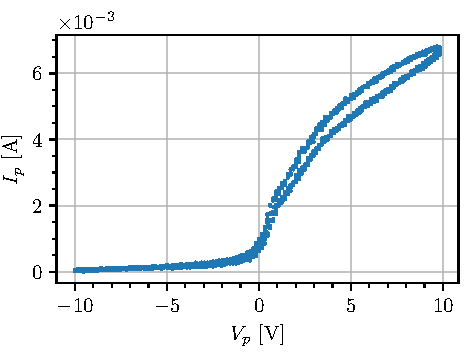
\includegraphics[scale=1]{../figures/hysteresis.pdf}\\
            \small $I$-$V$ curve acquired at $p = (7.2 \pm 0.1) \times 10^{-3}$ mbar and $\filamentcurrent = (55.5 \pm 0.1)$ A
        \end{center}

        \column{0.35\textwidth}
        \begin{center}
            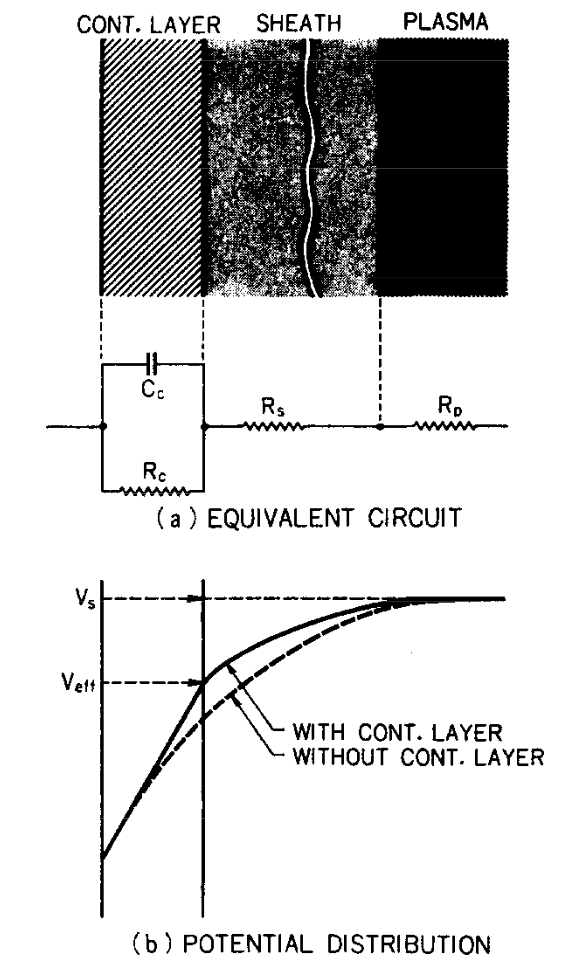
\includegraphics[width=3.5cm]{../figures/contamination_layer.png}\\
            \small Model for the contamination layer [12]
        \end{center}
        
    \end{columns}

\end{frame}


\begin{frame}{Possible further studies}
    \begin{itemize}
        \item Different probe geometry: complete 2D profile of the chamber
        \item Higher number of probes (e.g. an array)
        \item Mixtures of gas species
    \end{itemize}
\end{frame}


\end{document}
